\chapter{Design}
In this chapter we focus on how to implement what we have specified in the analysis chapter.
First, we describe our application's architecture.
Then, we discuss what technologies were considered for implementing the application, and which of the technologies were chosen and why.
We name our application "Choose well".

\section{Architecture}
\todo[inline]{add footnote}
We design our solution(footnote - from now on we will refer to the whole application as the solution as not to  confuse it with the applications it consists of) as multiple independent single-page applications for better modularity. 
One application is the guest dietary profile editor.
It allows a guest to set their dietary preferences like being allergic to something or being vegetarian.
Another application is the restaurant menu maker.
It serves for restaurant employees to specify their menu's contents.
Last application is the personalized menu viewer for restaurant guests.
It combines information gathered by the other applications to display personalized menus to guests. 
\todo[inline]{add figure number}
\todo[inline]{move bottom border a bit lower}
Figure x contains a depiction of our solution's architecture.

\begin{figure}[h]
  \centering
  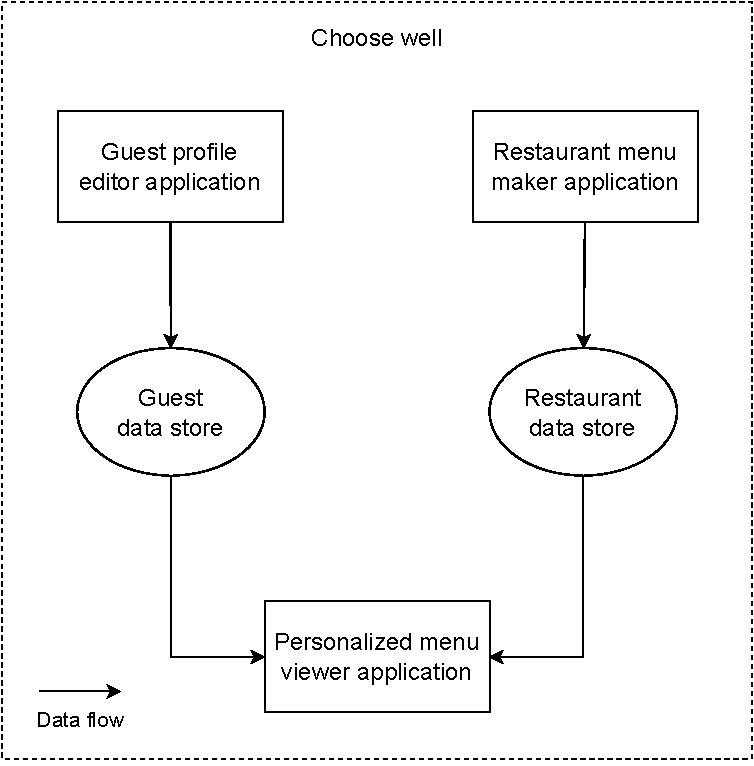
\includegraphics[width=0.62\linewidth]{master-thesis/img/architecture_data_flow.pdf}
  \caption{The solution's architecture}
\end{figure}

\section{Technological stack}
\todo[inline]{add links to technologies - footnotes, link to documentation of the technology}
This section contains an overview of considered tools for implementing the solution.
We also note which ones we chose and why.

\subsection*{User interface}
\todo[inline]{add link}
We chose \textbf{React} for developing the UI of the solution's applications.
This decision was made on the account that Solid is programmed for React and there even exists a Solid React SDK(link).

\subsection*{Programming language}
As for a programming language, JavaScript and TypeScript were considered.
Both languages are supported by React, and we chose \textbf{Typescript} because it adds type control to the programmer's code which makes it less error-prone.

\subsection*{Build tool}
/todo[inline]{add footnotes}
For the initial creation and building of applications during development, Create React App(footnote) and Vite(footnote) were considered.
We decided to choose \textbf{Vite} as it was recommended by a skilled Solid developer (footnote forum solid). 


\subsection*{Deployment}
\todo[inline]{add link to GH Pages doc}
For deployment the \textbf{GitHub Pages}(link) technology is used as the application's repositories already reside on GitHub.


\subsection*{Package manager}
The \textbf{npm} package manager is used for handling packages in our projects.
We chose npm because it is widely used and provides what we need for development of the applications. 


\subsection*{Responsive design}
Two options were considered in this topic: Bootstrap and Material UI.
We opted for \textbf{Bootstrap} as it is easy to use and is well documented.


\subsection*{Persistence}
We decided to use the \textbf{Solid} technology for storing the users' data. 

\subsection*{Documentation}
\todo[inline]{add links to docs in footnote}
Programmer and administrator documentation is made using \textbf{GitHub markdown} in the projects' public repositories.
User documentation is in a form of a webpage(link) which is hosted on \textbf{GitHub Pages}.

\subsection*{Authentication}
For authentication purposes, the Inrupt's solid-client JavaScript library is used.
We also use the Inrupt's Solid React SDK which contains a Login component which uses the aforementioned library implicitly.
